%                      Code_Saturne version 1.3
%                      ------------------------
%
%     This file is part of the Code_Saturne Kernel, element of the
%     Code_Saturne CFD tool.
%
%     Copyright (C) 1998-2007 EDF S.A., France
%
%     contact: saturne-support@edf.fr
%
%     The Code_Saturne Kernel is free software; you can redistribute it
%     and/or modify it under the terms of the GNU General Public License
%     as published by the Free Software Foundation; either version 2 of
%     the License, or (at your option) any later version.
%
%     The Code_Saturne Kernel is distributed in the hope that it will be
%     useful, but WITHOUT ANY WARRANTY; without even the implied warranty
%     of MERCHANTABILITY or FITNESS FOR A PARTICULAR PURPOSE.  See the
%     GNU General Public License for more details.
%
%     You should have received a copy of the GNU General Public License
%     along with the Code_Saturne Kernel; if not, write to the
%     Free Software Foundation, Inc.,
%     51 Franklin St, Fifth Floor,
%     Boston, MA  02110-1301  USA
%
%-----------------------------------------------------------------------
\newpage
%-----------------------------------------------------------------------------------------------------------------
\section{CASE 3:  Time dependent boundary conditions and variable fluid density}
%-----------------------------------------------------------------------------------------------------------------
In this case some boundary conditions will be time dependent and some physycal
characteristics of the fluid will be dependent on the temperature.

        \subsection{Calculation options}
%-----------------------------------------

The options for this case are the same as in case 2, except for the variable fluid density:
\begin{itemize}
\renewcommand{\labelitemi}{$\rightarrow$}
        \item Flow type: unsteady flow
        \item Time step: uniform and constant
        \item Turbulence model: $k-\epsilon$
        \item Scalar(s): 1 - temperature\\
      \hspace*{1.6cm} 2 - passive scalar
        \item Physical properties: uniform and constant (except density)
        \item Management of monitoring points
\end{itemize}


        \subsection{Initial and boundary conditions}
%---------------------------------------------------

\begin{itemize}
\renewcommand{\labelitemi}{$\rightarrow$}
        \item Initialization: 20\degresC\ for temperature (default value) \\
        \hspace*{2.1cm}        10 for the passive scalar
\end{itemize}

The boundary conditions are defined in the user interface and depend on the
boundary zone. The time dependence of the temperature boundary condition implies
the use of a Fortran user routine (see below).

\begin{itemize}
        \item {\bfseries Flow inlet}: Dirichlet condition, an inlet velocity of
$1\ m.s^{-1}$, a time dependent inlet temperature and a value of 200 for the
passive scalar are imposed
        \item {\bfseries Outlet}: default value
        \item {\bfseries Walls}: velocity, pressure and thermal scalar: default value \\
                    \hspace*{1.25cm} passive scalar: different conditions
depending on the color and geometric parameters
\end{itemize}

The boundary conditions for the passive scalar are identical as in case 2,
as specified in the following table:

\begin{center}
\begin{tabular}{|c|c|c|}
\hline
Wall & Nature & Value \\
\hline
wall\_1 & Dirichlet  & 0 \\
\hline
wall\_2 & Dirichlet  & 5 \\
\hline
wall\_3 & Dirichlet  & 0 \\
\hline
wall\_4 & Dirichlet  & 25 \\
\hline
wall\_5 & Dirichlet  & 320 \\
\hline
wall\_6 & Dirichlet  & 40 \\
\hline
\end{tabular}
\end{center}

The ``wall\_1'' to ``wall\_6'' regions are defined as follows, through color
references and geometric localization:
\begin{center}
\begin{tabular}{c|c}
Label & Color and geometric parameters \\
\hline
wall\_1 & 24 and $0.1\leqslant X$ and $X\leqslant 0.5$ \\
wall\_2 & 2 or 3 \\
wall\_3 & 4 or 7 or 21 or 22 or 23 \\
wall\_4 & 6 and $Y>1$ \\
wall\_5 & 6 and $Y\leqslant1$ \\
wall\_6 & 31 or 33 \\
\end{tabular}
\end{center}

Figure \ref{figante23} shows the colors used for boundary conditions and
table \ref{tabante31} defines the correspondance between the colors and
the type of boundary condition to use.

\begin{table}[htp]
\begin{center}
\begin{tabular}{|c|c|}
\hline
Colors & Conditions \\
\hline
1 & Inlet \\
\hline
34 & Outlet \\
\hline
2 3 4 6 7 21 22 23 31 33 & Wall \\
\hline
24 for $0.1 \leq X \leq 0.5$ & Wall \\
\hline
8 9 28 29 38 39 & Symmetry \\
\hline
\end{tabular}
\caption{Boundary faces colors and associated references}
\label{tabante31}
\end{center}
\end{table}


        \subsection{Parameters}
%------------------------------

All the parameter necessary to this study can be defined through the Graphical
Interface, except the time dependent boundary conditions and the variable
density that have to be specified in user routines.

\begin{center}
\begin{tabular}{|l|c|}
\hline
\multicolumn{2}{|c|}{Parameters of calculation control} \\
\hline
Number of iterations & $300$ \\
\hline
Reference time step & $0.05$ \\
\hline
Output period for post-processing files& $2$ \\
\hline
\end{tabular}\\
\end{center}

In order to paste the separate meshes into a single domain, colors 5, 24 and 32
will have to be pasted through the Graphical Interface.


        \subsection{User routines}
%---------------------------------

The following routines have to be copied from the folder FORT/USER/base into the
folder FORT\footnote{only when they appear in the FORT directory will they be
taken into account by the code}: usclim.F and usphyv.F.

$\bullet$ {\bfseries usclim.F}\\
This routine allows to define advanced boundary conditions on the boundary
faces. Even if usclim.F is used, all boundary conditions have to be defined in
the Graphical User Interface. Only the conditions that differ from this first
definition need appear in usclim.F. The boundary conditions defined in usclim.F
will replace those specified in the Graphical Interface.

In this case, the temperature at entry is supposed variable in time, following
the law:
\begin{equation}
\left\{\begin{array}{ll}
T = 20 + 100t & \text{for }0\leqslant t \leqslant 3.8\\
T = 400 & \text{for } t > 3.8
\end{array}\right.
\end{equation}
where $T$ is the temperature in \degresC\ and $t$ is the time in $s$.


\begin{figure}[h!]
\begin{center}
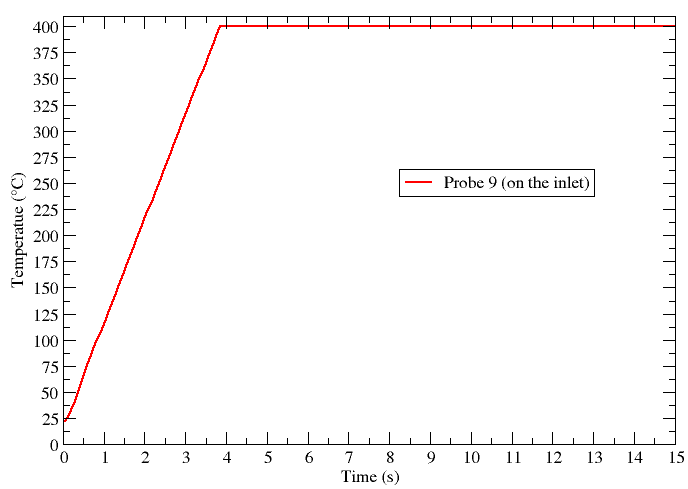
\includegraphics[width=9cm,height=6.4cm]{\repgraphics/probe9.png}
\caption{Time evolution of the temperature at inlet}
\label{figp9_e3}
\end{center}
\end{figure}


$\bullet$ {\bfseries usphyv.F}\\
This routine allows to specify variable physical properties, density in
particular. In this case, the variation law given as an example in the routine
will be appropriate:
\begin{equation}
\rho = T.(A.T + B) + C
\end{equation}
where $\rho$ is the density, $T$ is the temperature, $A = -4.0668\times10^{-3}$,
$B =-5.0754\times 10^{-2}$ and $C = 1\,000.9$

\textbf{Note:} in the example routine, the example is protected by a test to prevent any
undesired use. Do not forget to deactivate it.

In order for the variable density to have an effect on the flow, gravity must be
set to a non-zero value. $\vect{g} = -9.81 \vect{e}_y$ will be specified in the
Graphical Interface.

        \subsection{Output management}
%-------------------------------------

The output management is the same as in case 2, except that a nineth monitoring
point will be added, just at the entry, to monitor the temperature evolution at inlet.

\begin{figure}[htp]
\parbox{8cm}{%
\centerline{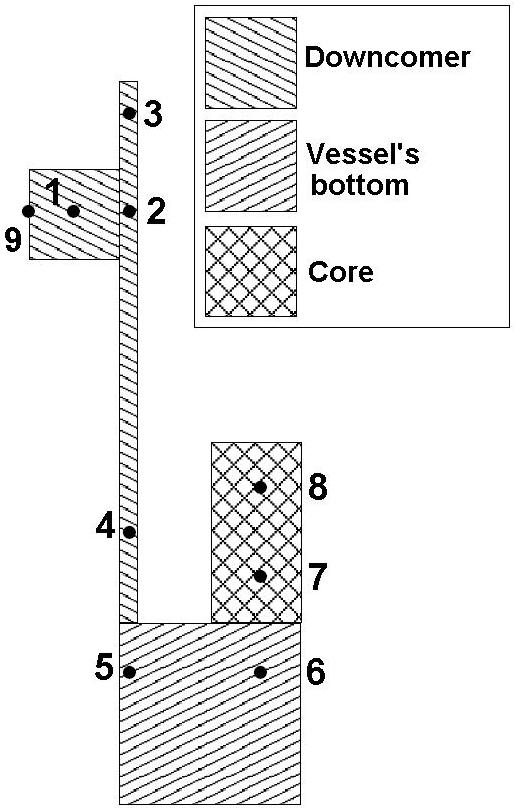
\includegraphics[width=4cm,height=6.8cm]{\repgraphics/fig08.jpg}}}
\parbox{7cm}{%
\begin{center}
\begin{tabular}{|c|c|c|c|}
\hline
Points & X(m) & Y(m) & Z(m)\\
\hline
1 & -0.25 & 2.25 & 0 \\
\hline
2 & 0.05 & 2.25 & 0 \\
\hline
3 & 0.05 & 2.75 & 0 \\
\hline
4 & 0.05 & 0.5 & 0 \\
\hline
5 & 0.05 & -0.25 & 0 \\
\hline
6 & 0.75 & -0.25 & 0 \\
\hline
7 & 0.75 & 0.25 & 0 \\
\hline
8 & 0.75 & 0.75 & 0 \\
\hline
9 & -0.5 & 2.25 & 0 \\
\hline
\end{tabular}
\end{center}
}
\caption{Position and coordinates of probes in the full domain}
\label{figante32}
\end{figure}

In this case, the {\itshape Pressure}, the {\itshape Tubulent energy} and the
{\itshape Dissipation} will be removed from the listing file.

The {\itshape Courant number} (CFL) and {\itshape Fourier number} will be
removed from the
post-processing results\footnote{this can be very useful to save some disk space
if some variables are of no interest, as post-processing files can be large}.

Eventually, probes will be defined for chronological records, folowing the data
given in figure \ref{figante25}. Then the {\itshape total pressure} will be
deactivated from all probes and the {\itshape Velocity U} will be only activated
on probes  1, 2, 6, 7 and 8.


In addition the domain boundary will be post-processed. This allows to check the
boundary conditions, and especially that of the temperature and passive scalar.


        \subsection{Calculation restart}
%---------------------------------------

After the first run, the calculation will be continued for another 400 time
steps. The calculation restart is managed through the Graphical Interface.


        \subsection{Results}
%---------------------------
Figure \ref{fige3_e3} shows the time evolution of temperature recorded on each
monitoring probe.
\begin{figure}[hb]
\begin{center}
\begin{tabular}{cc}
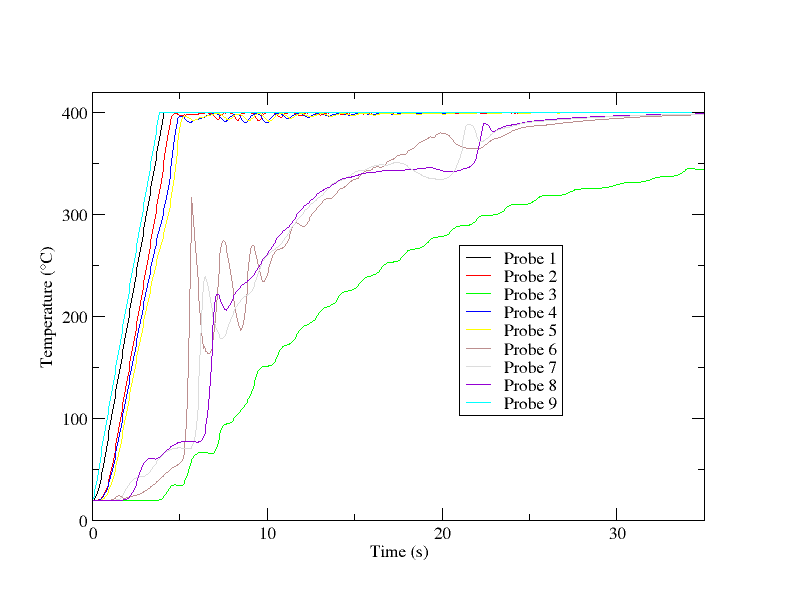
\includegraphics[width=11cm]{\repgraphics/evotemp_case3.png} \\
\end{tabular}
\caption{Time evolution of temperature at monitoring probes for case 3}
\label{fige3_e3}
\end{center}
\end{figure}

Figure \ref{fige1_e3} shows the velocity fields colored by temperature in the
first run of calculation. Figure \ref{fige2_e3} shows the velocity fields in the
second calculation (restart of the first one).

\begin{figure}
\begin{center}
\begin{tabular}{cc}
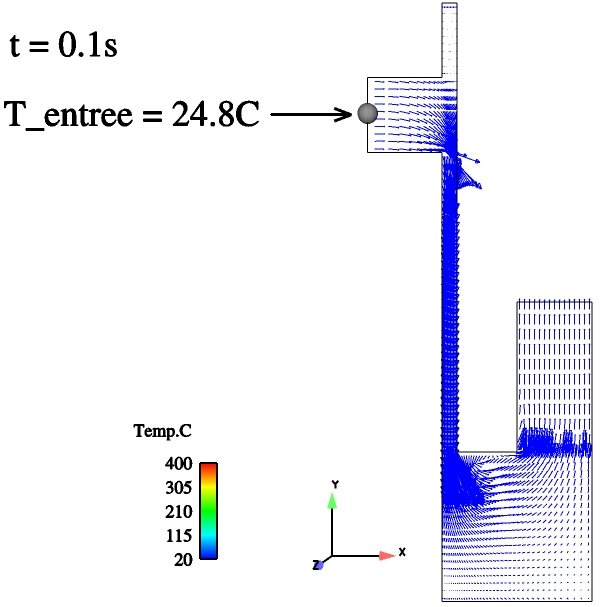
\includegraphics[height=6cm]{\repgraphics/case3_p1.jpg} &
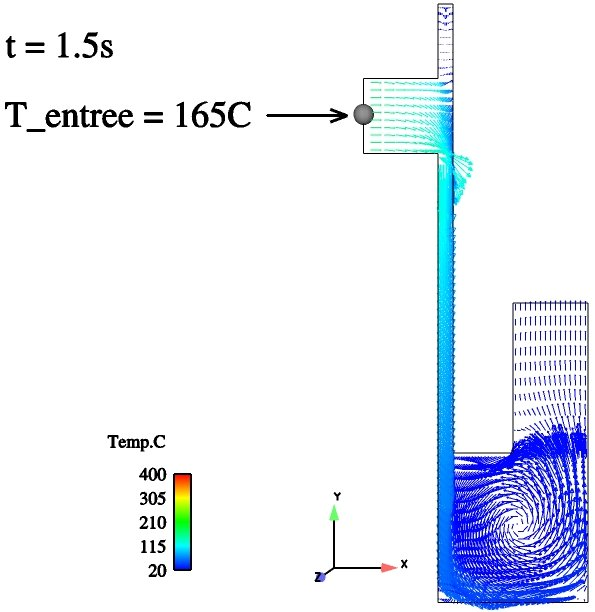
\includegraphics[height=6cm]{\repgraphics/case3_p2.jpg} \\
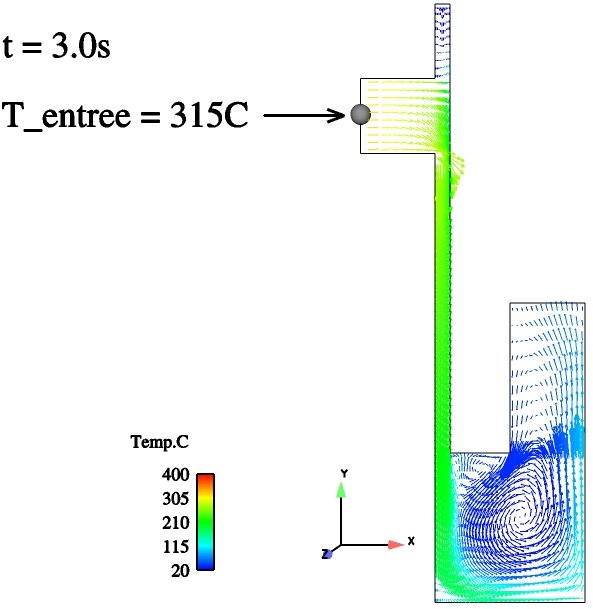
\includegraphics[height=6cm]{\repgraphics/case3_p3.jpg} &
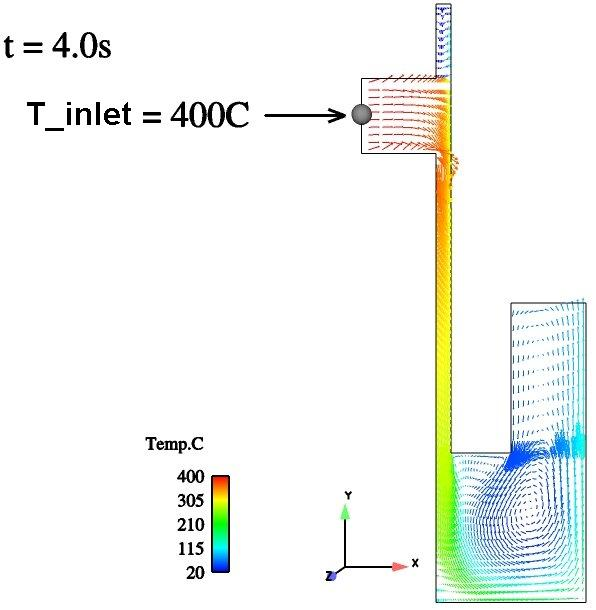
\includegraphics[height=6cm]{\repgraphics/case3_p4.jpg} \\
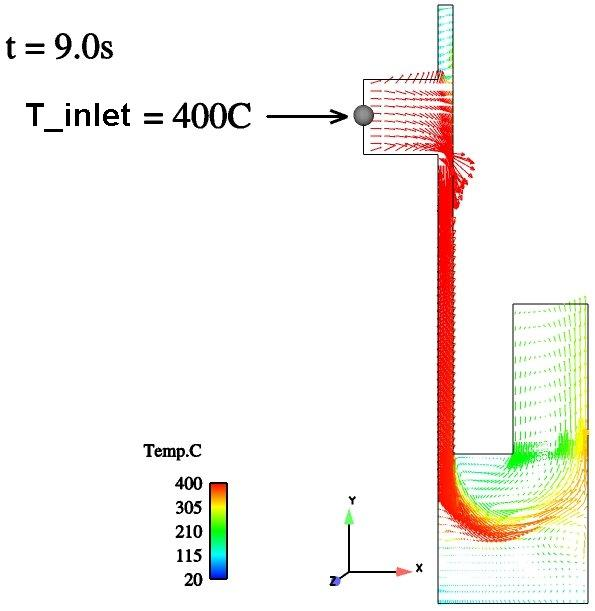
\includegraphics[height=6cm]{\repgraphics/case3_p5.jpg} &
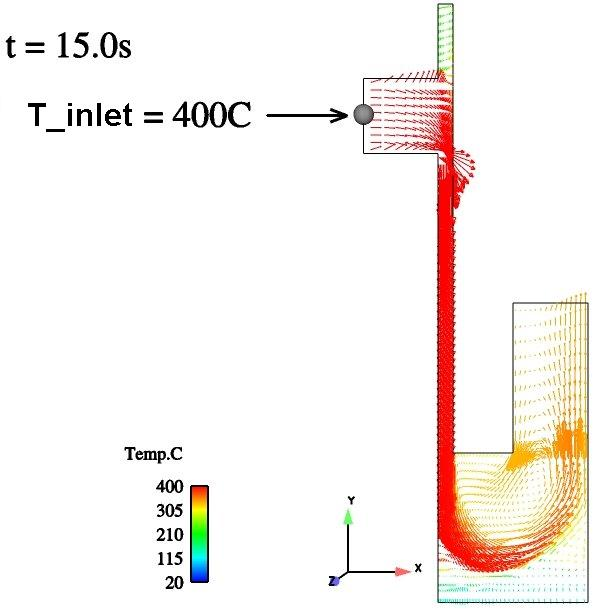
\includegraphics[height=6cm]{\repgraphics/case3_p6.jpg} \\
\end{tabular}
\caption{Water velocity field colored by temperature and inlet temperature value
at different time steps (first calculation)}
\label{fige1_e3}
\end{center}
\end{figure}


\begin{figure}
\begin{center}
\begin{tabular}{cc}
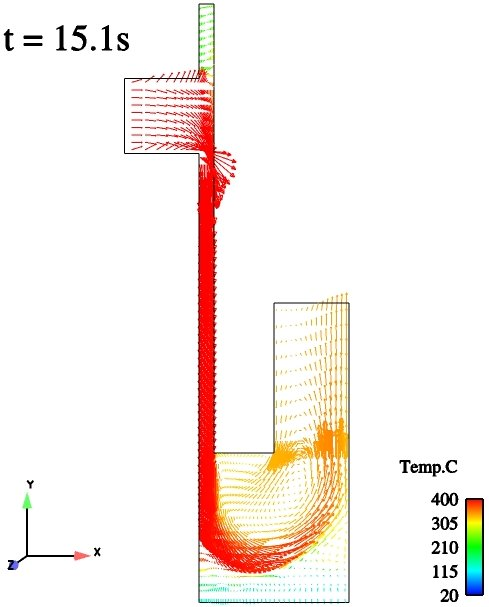
\includegraphics[height=7.5cm]{\repgraphics/case3_p7.jpg} &
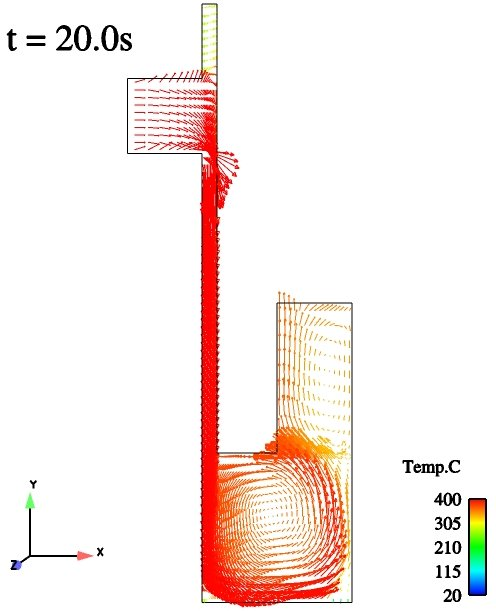
\includegraphics[height=7.5cm]{\repgraphics/case3_p8.jpg} \\
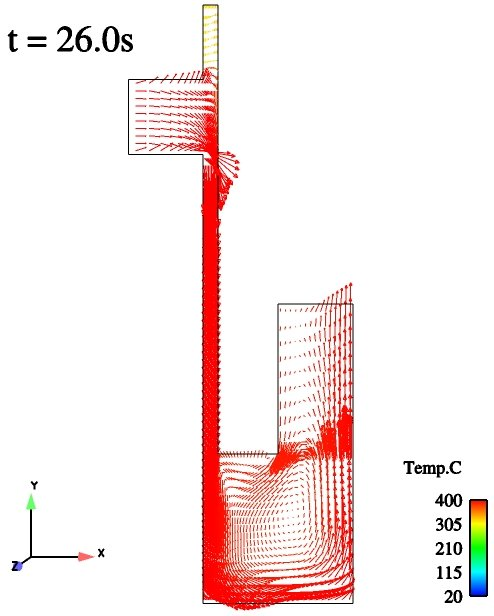
\includegraphics[height=7.5cm]{\repgraphics/case3_p9.jpg} &
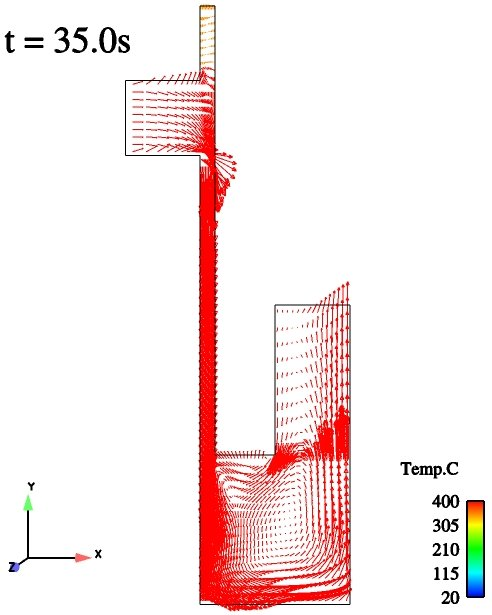
\includegraphics[height=7.5cm]{\repgraphics/case3_p10.jpg} \\
\end{tabular}
\caption{Water velocity field colored by temperature and inlet temperature value
at different time steps (second calculation)}
\label{fige2_e3}
\end{center}
\end{figure}






